\documentclass{article}

% Chinese Support using xeCJK
% \usepackage{xeCJK}
% \setCJKmainfont{SimSun}

% Chinese Support using CTeX
\usepackage{ctex}

% Math Support
\usepackage{amsmath}
\usepackage{amsfonts}
\usepackage{amssymb}
\usepackage{wasysym}
\newcommand{\angstrom}{\text{\normalfont\AA}}

% Graphics Support
\usepackage{graphicx}
\usepackage{float}

% Reduced page margin
\usepackage{geometry}
\geometry{a4paper,scale=0.8}

\usepackage{caption}
\usepackage{subcaption}

% d and e should be math operators
\newcommand*{\dif}{\mathop{}\!\mathrm{d}}
\newcommand*{\md}{\mathop{}\!\mathrm{d}}
\newcommand*{\me}{\mathrm{e}}

% No indent for each paragraph
% \usepackage{parskip}
% \setlength{\parindent}{0cm}

% Bold style for Greek letters
\usepackage{bm}
\let\Oldmathbf\mathbf
\renewcommand{\mathbf}[1]{\boldsymbol{\Oldmathbf{#1}}}

% More space for dfrac in cell
\usepackage{cellspace}
\setlength{\cellspacetoplimit}{5pt}
\setlength{\cellspacebottomlimit}{5pt}

% SI units
\newcommand{\si}[1]{\  \mathrm{#1}}

% Multi-line author information
\usepackage{authblk}
\author{物理(4+4)1801 \quad  胡喜平 \quad U201811966}
\affil{个人网站 https://hxp.plus/ \quad 电子邮件 hxp201406@gmail.com}

\usepackage{pdfpages}

\title{近代物理实验预习笔记——电路综合实验}

\begin{document}

\maketitle

\section{实验内容}

\begin{itemize}
\item 设计一个中心频率在$100 \si{kHz}$的带通滤波器,测量传递函数,比较电阻对实验结果的影响。
\item 测量运算放大器的输入失调电压,输入失调电流,开环电压放大倍数,共模抑制比。
\item 设计一个电路,输出为$U_O = 0.5 U_{i1} + 0.5 U_{i2} - U_{i3}$,输入五组输入电压验证。
\item 搭建积分运算电路,输入$1 \si{kHZ}$的方波信号,记录输入输出波形,在不同频率下比较连接和不连接$R_f$有何不同。
\item 搭建微分运算电路,输入$1 \si{kHZ}$方波、三角波信号,记录输入输出波形,在不同频率下移去$R$和$C_f$,观察波形变化。
\item 设计RC正弦波电路,测量波形,计算频率振幅,与设计的振幅频率比较。
\item 设计占空比$1/3$的矩形波电路,连线后接入示波器,画出调好的波形图,计算$T_k$和$T$,与设计值相比较。
\item 设计矩形-三角波电路,要求占空比连续可调。
\end{itemize}

在实验开始前,将设计好的实验电路进行计算机模拟是一个很好的选择。计算机模拟能初步检验电路设计是否出现了问题,并且节约实验现场调试电路问题花费的时间和材料。以下是我设计的电路和在计算机中模拟运行的结果。实验中大致应当出现这些模拟出来的现象。

之后的按照先后顺序分别是:

\begin{itemize}
\item 带通滤波器
\item 加减法电路
\item 积分电路
\item 微分电路
\item RC正弦波电路
\item 矩形波电路
\item 矩形-三角波电路
\end{itemize}

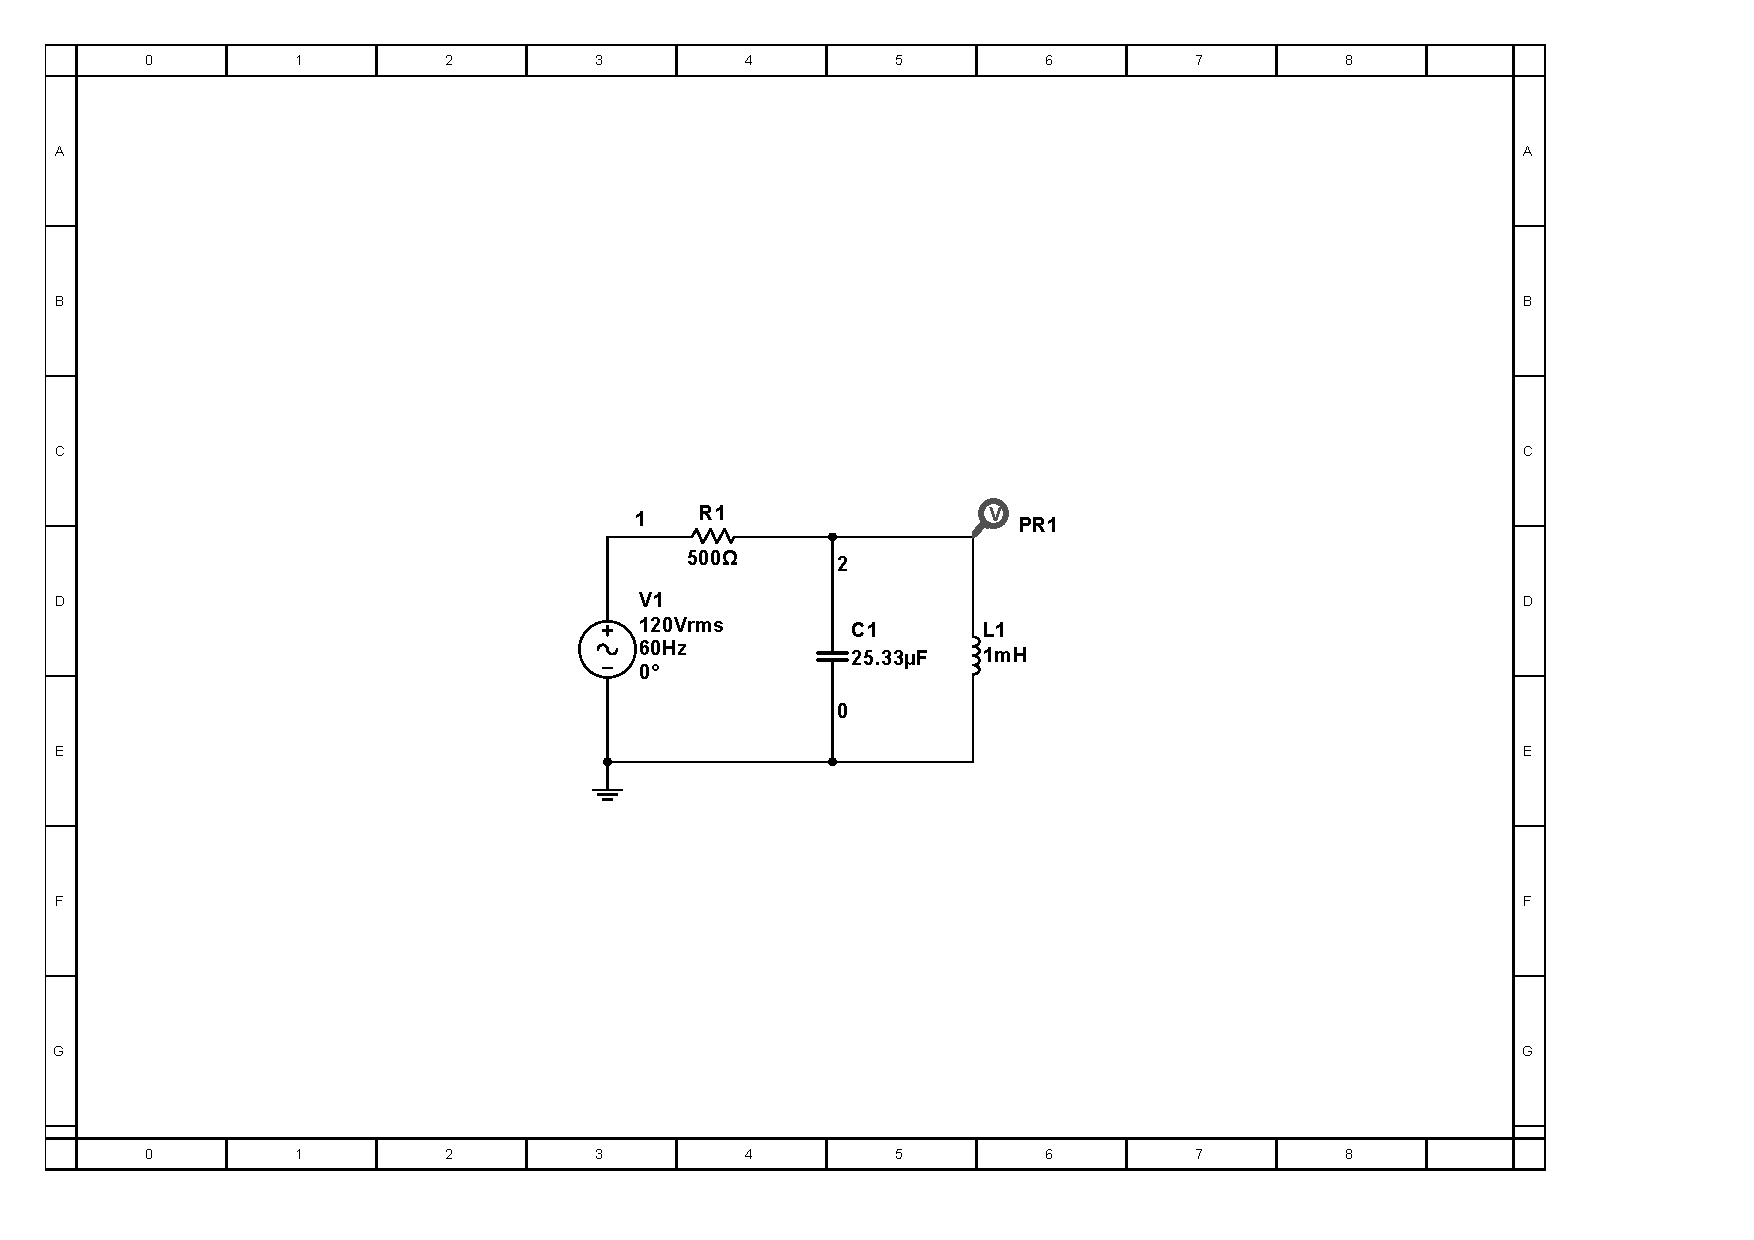
\includepdf[pages={1},angle=90]{/home/hxp/Notes/Physics_Experiment/近代物理实验——电路设计/带通滤波器/带通滤波器电路图.pdf}

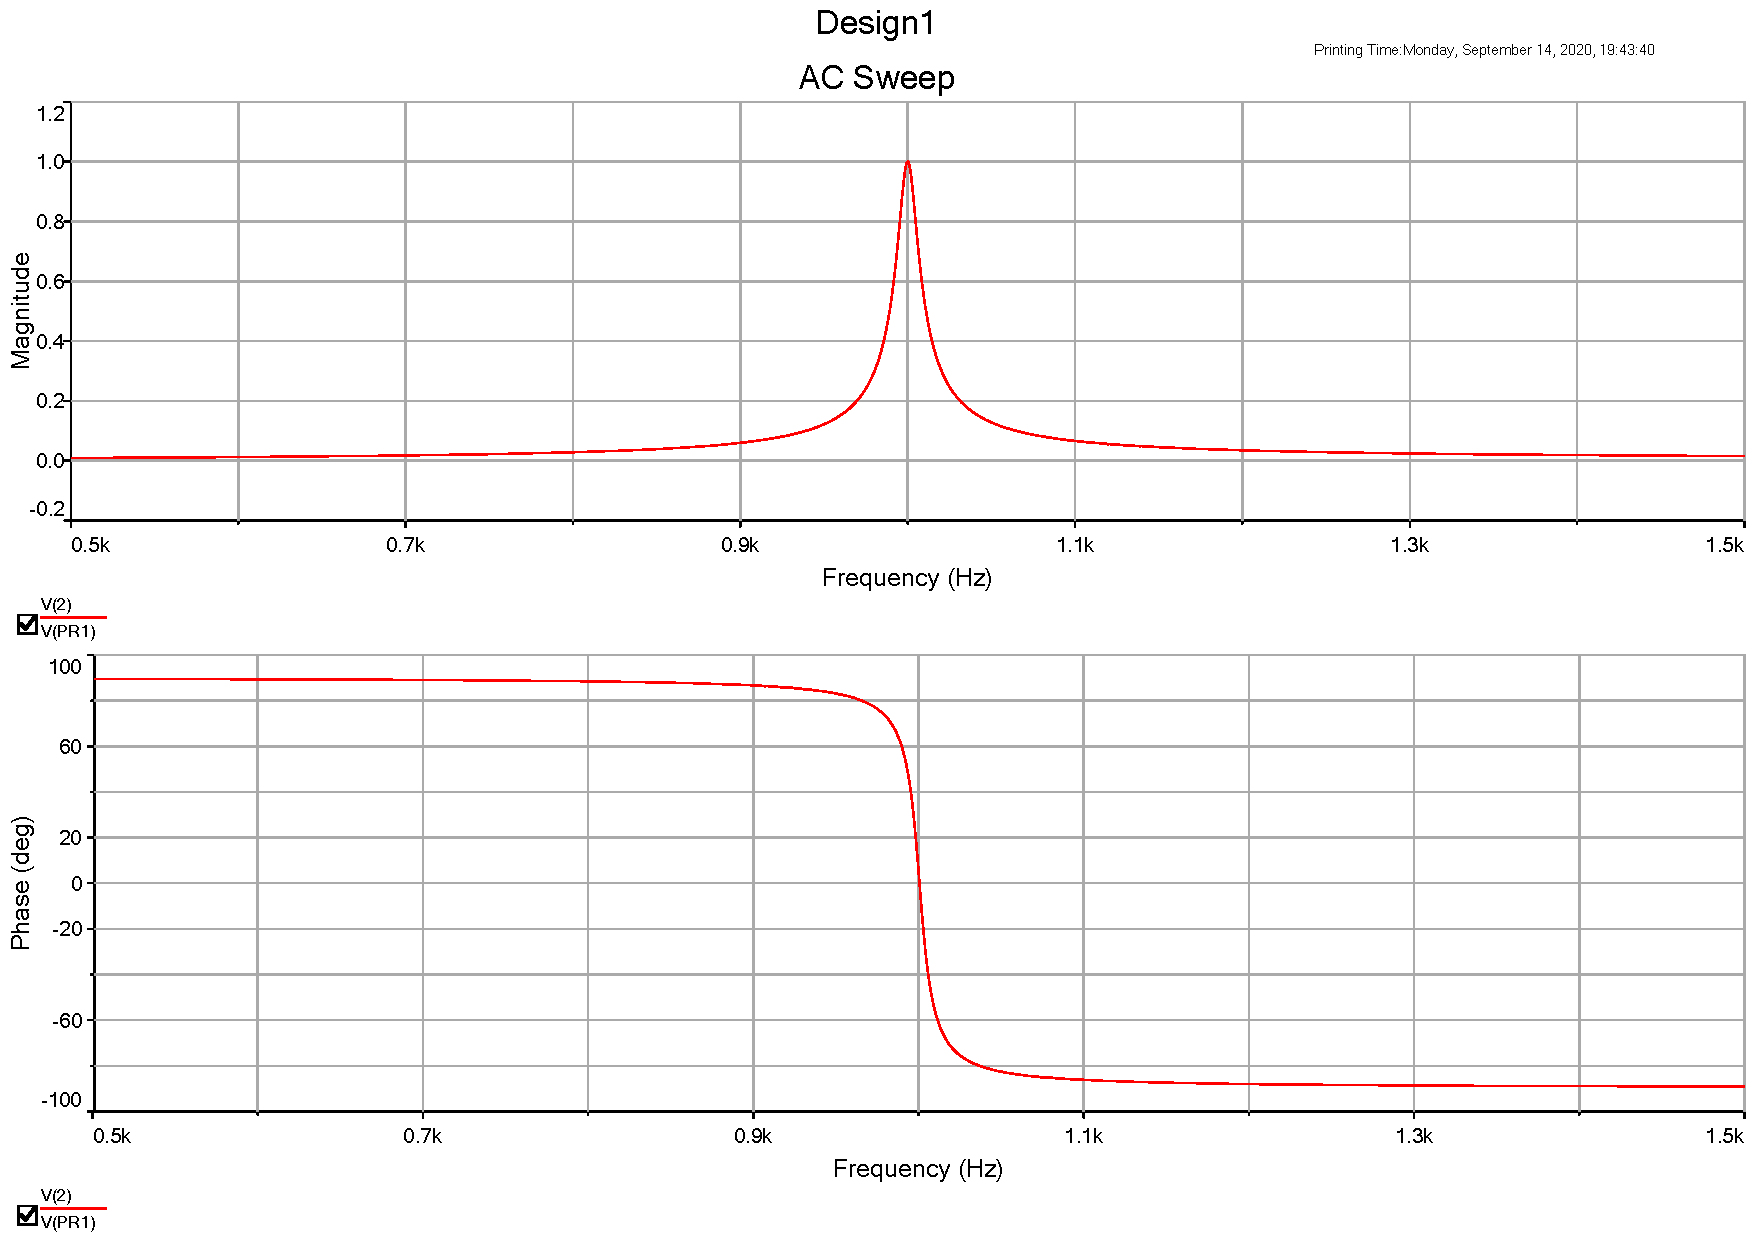
\includepdf[pages={1},angle=90]{/home/hxp/Notes/Physics_Experiment/近代物理实验——电路设计/带通滤波器/带通滤波器频率相应.pdf}

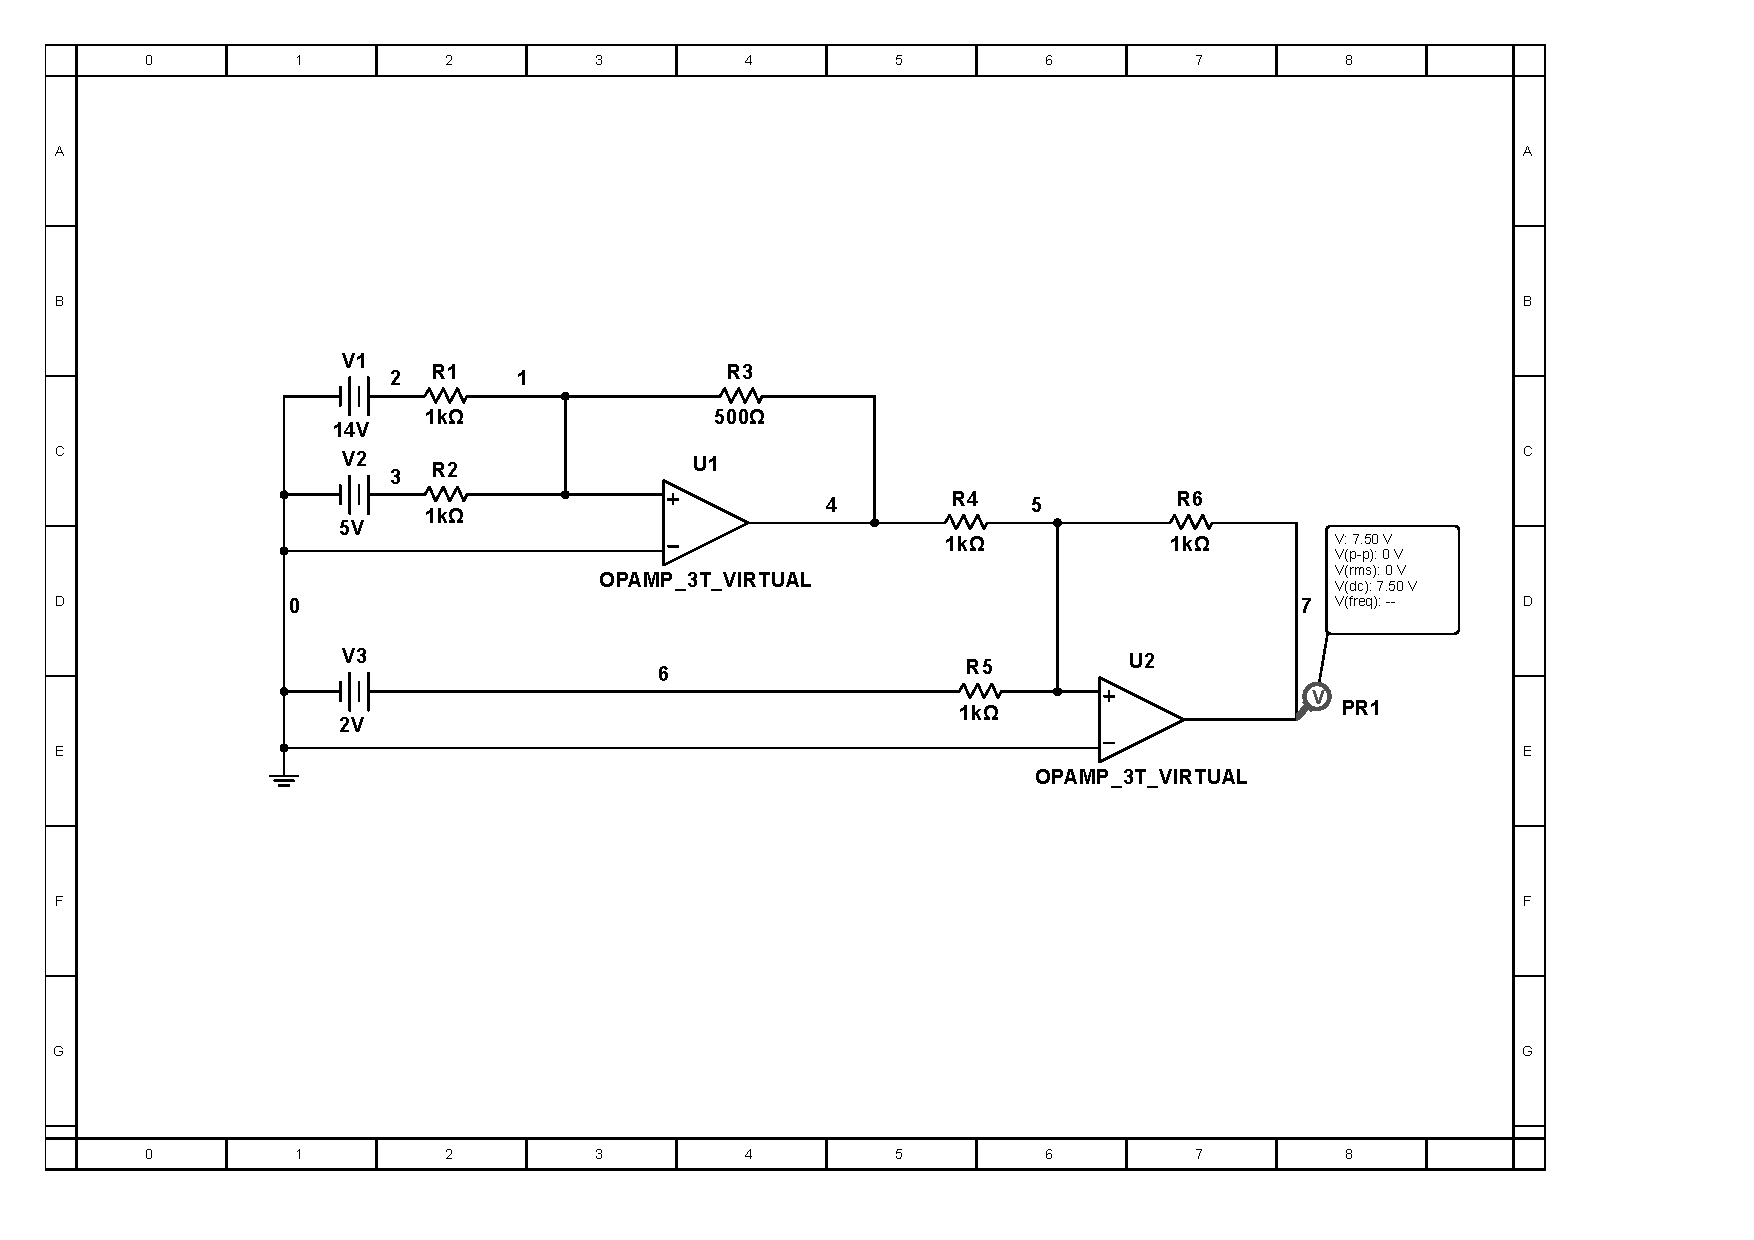
\includepdf[pages={1},angle=90]{/home/hxp/Notes/Physics_Experiment/近代物理实验——电路设计/加减法电路/加减法电路电路图.pdf}

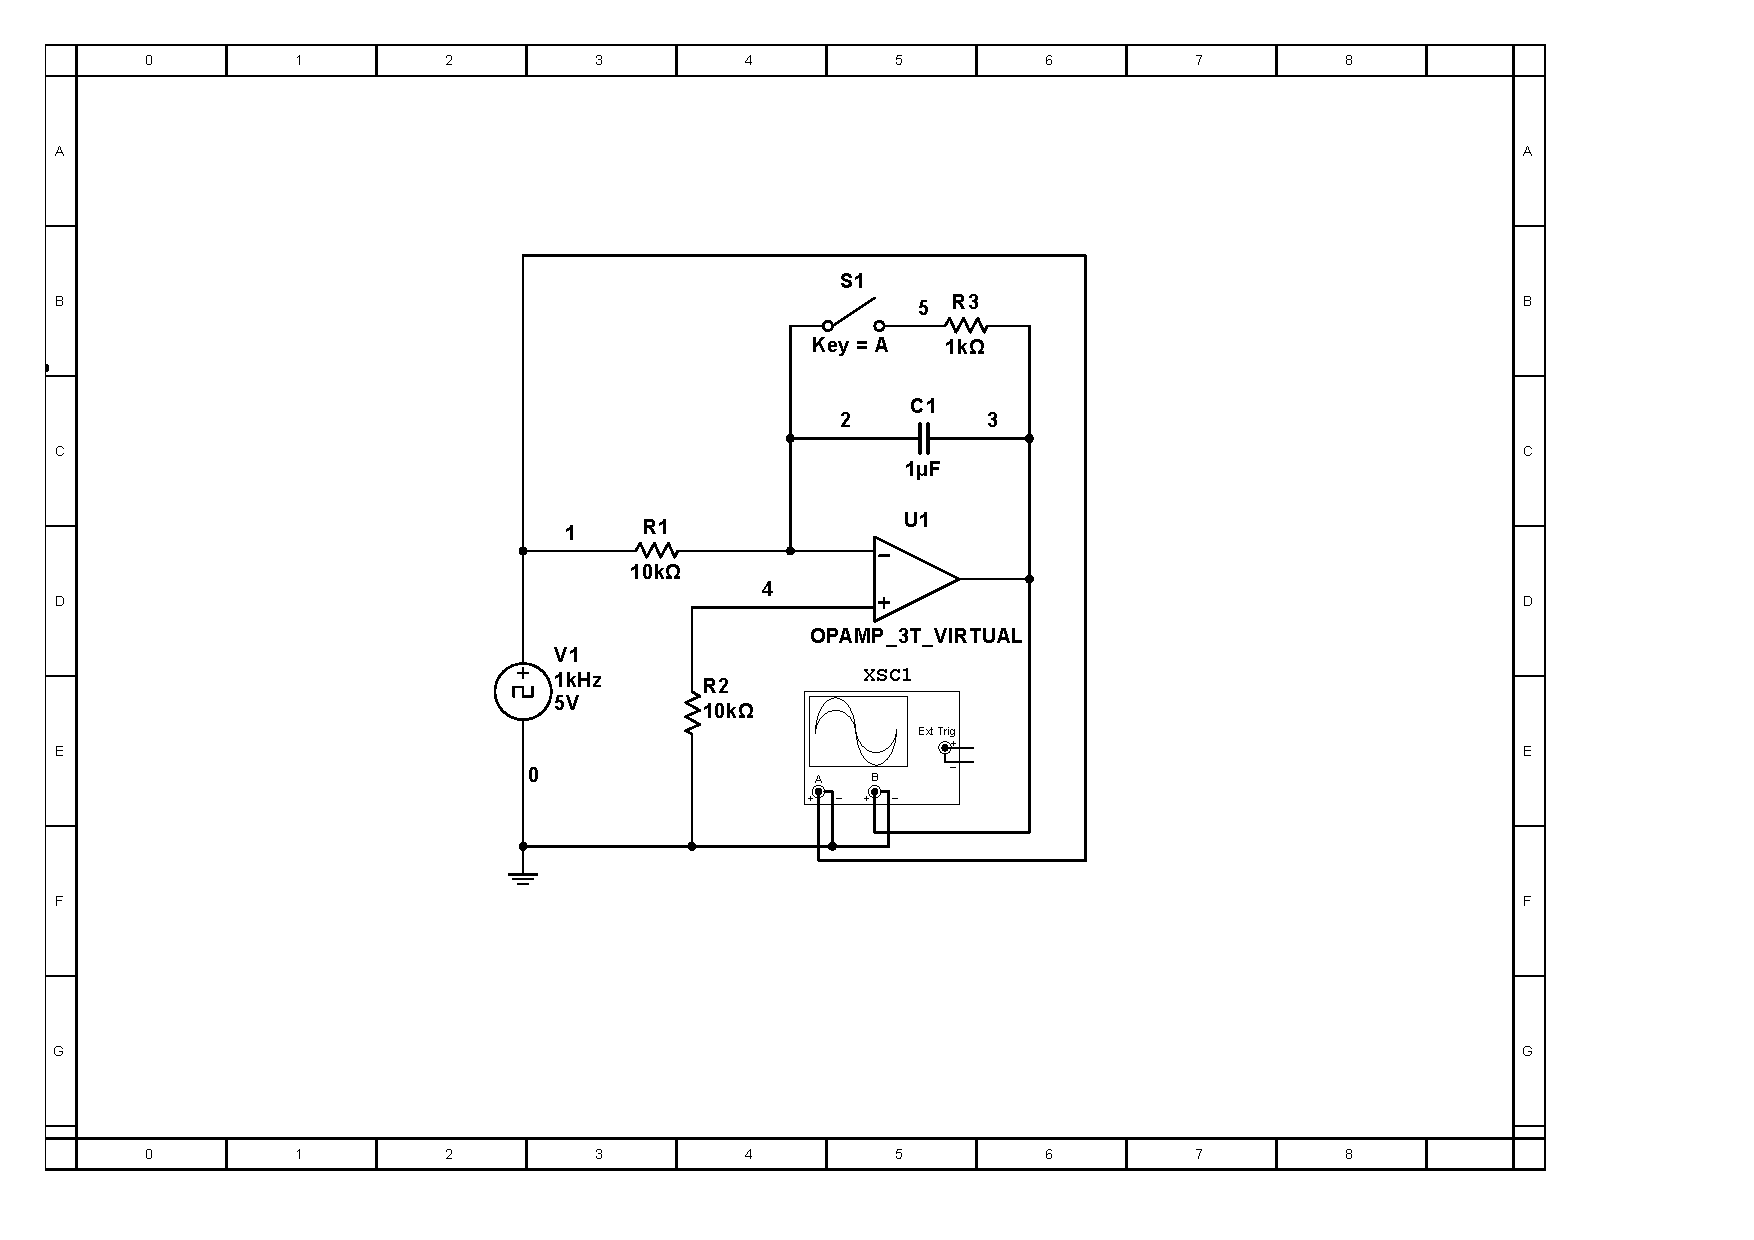
\includepdf[pages={1},angle=90]{/home/hxp/Notes/Physics_Experiment/近代物理实验——电路设计/积分电路/积分电路电路图.pdf}

\begin{figure}[H]
  \centering
  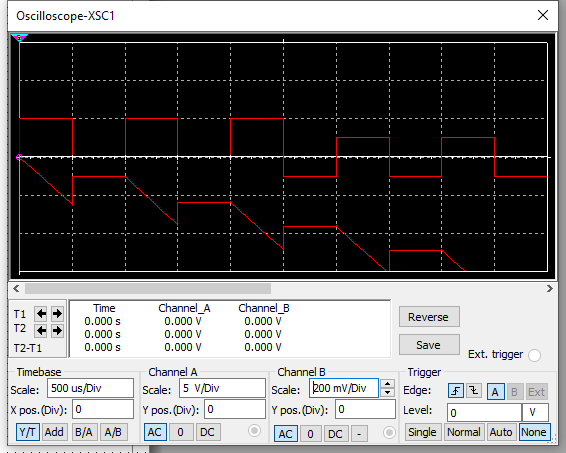
\includegraphics[width=0.75\linewidth]{/home/hxp/Notes/Physics_Experiment/近代物理实验——电路设计/积分电路/积分电路无Rf.png}
  \caption{积分电路无Rf}
\end{figure}

\begin{figure}[H]
  \centering
  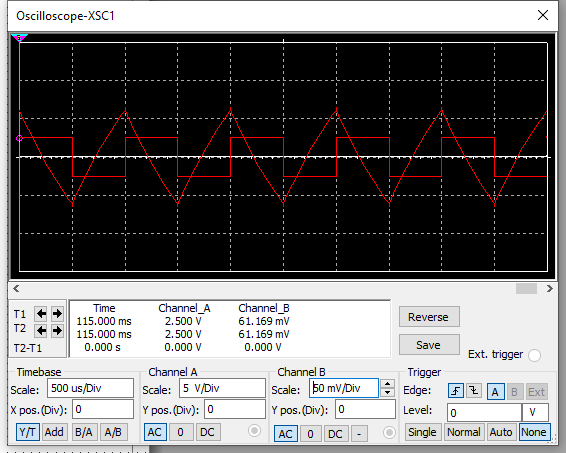
\includegraphics[width=0.75\linewidth]{/home/hxp/Notes/Physics_Experiment/近代物理实验——电路设计/积分电路/积分电路有Rf.png}
  \caption{积分电路有Rf}
\end{figure}

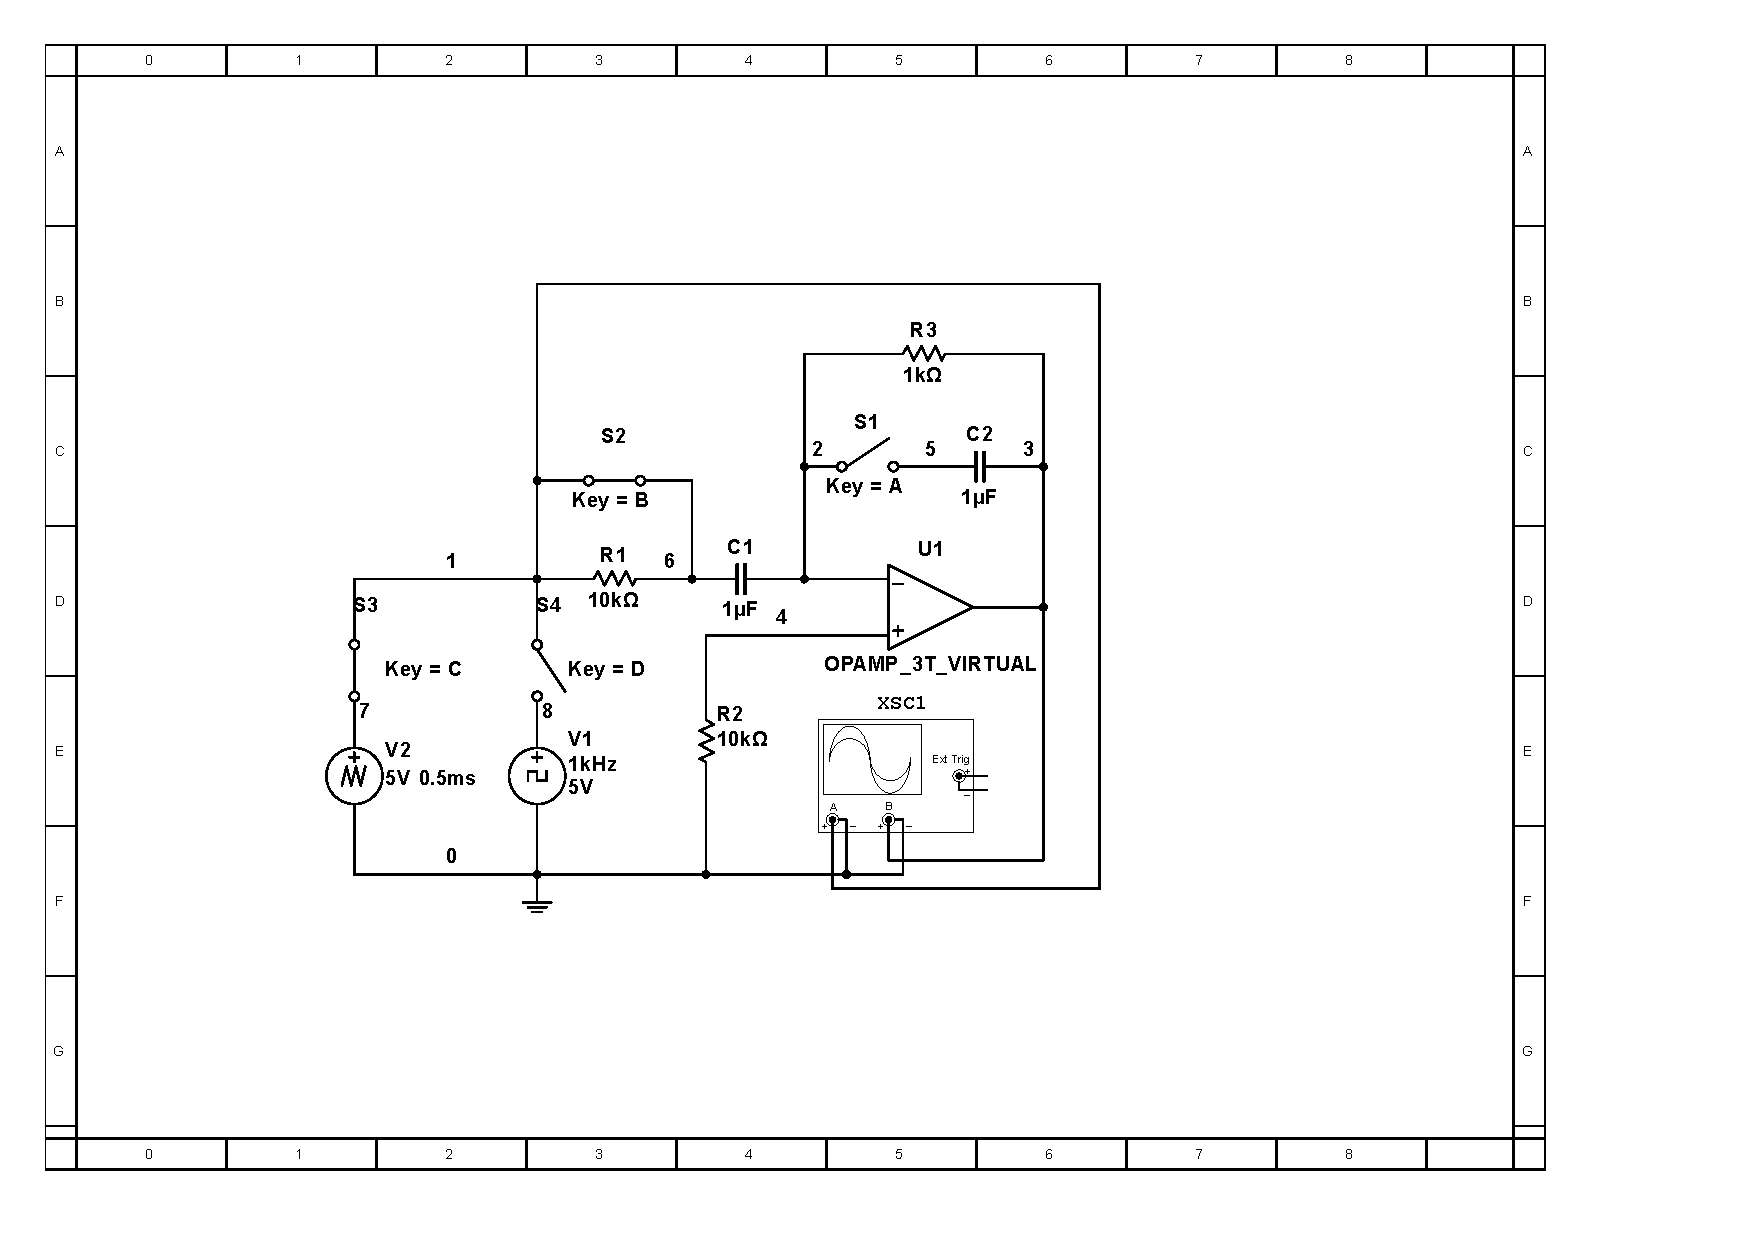
\includepdf[pages={1},angle=90]{/home/hxp/Notes/Physics_Experiment/近代物理实验——电路设计/微分电路/微分电路电路图.pdf}

\begin{figure}[H]
  \centering
  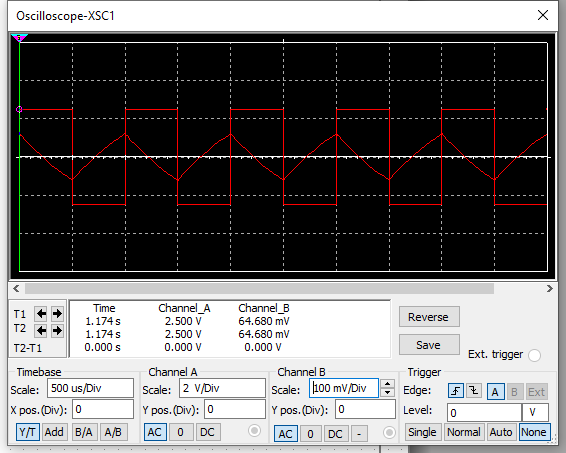
\includegraphics[width=0.75\linewidth]{/home/hxp/Notes/Physics_Experiment/近代物理实验——电路设计/微分电路/微分电路方波有电阻有电容.png}
  \caption{微分电路方波有电阻有电容}
\end{figure}

\begin{figure}[H]
  \centering
  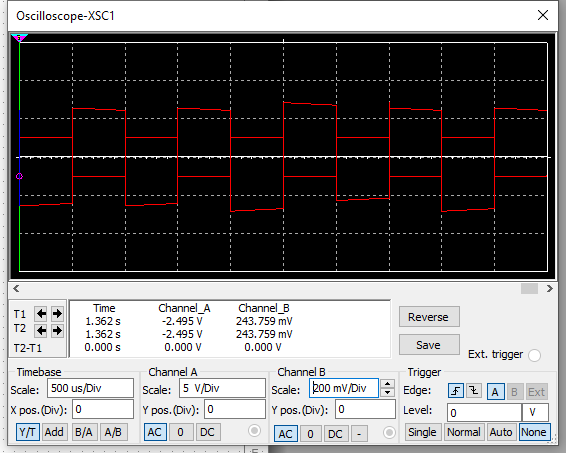
\includegraphics[width=0.75\linewidth]{/home/hxp/Notes/Physics_Experiment/近代物理实验——电路设计/微分电路/微分电路方波有电阻无电容.png}
  \caption{微分电路方波有电阻无电容}
\end{figure}

\begin{figure}[H]
  \centering
  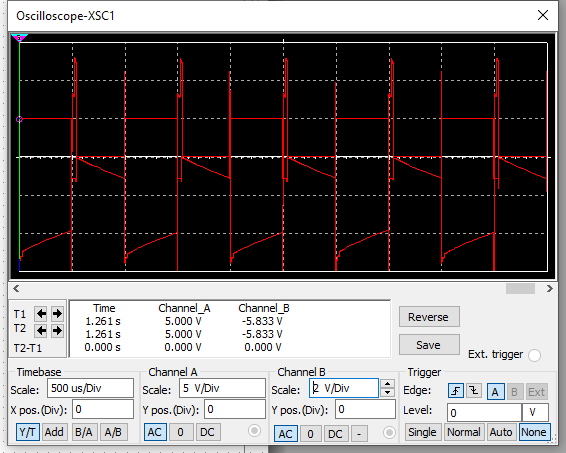
\includegraphics[width=0.75\linewidth]{/home/hxp/Notes/Physics_Experiment/近代物理实验——电路设计/微分电路/微分电路方波无电阻有电容.png}
  \caption{微分电路方波无电阻有电容}
\end{figure}

\begin{figure}[H]
  \centering
  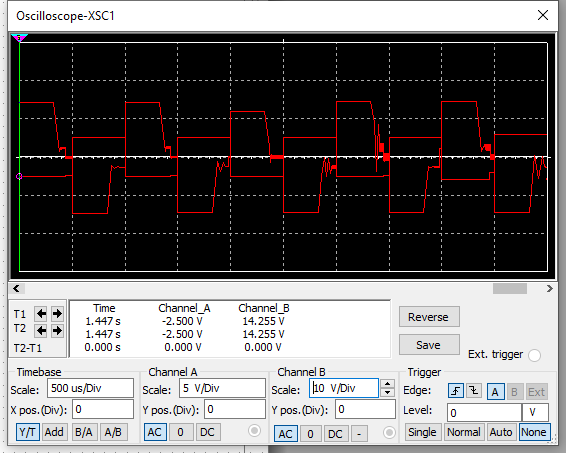
\includegraphics[width=0.75\linewidth]{/home/hxp/Notes/Physics_Experiment/近代物理实验——电路设计/微分电路/微分电路方波无电阻无电容.png}
  \caption{微分电路方波无电阻无电容}
\end{figure}

\begin{figure}[H]
  \centering
  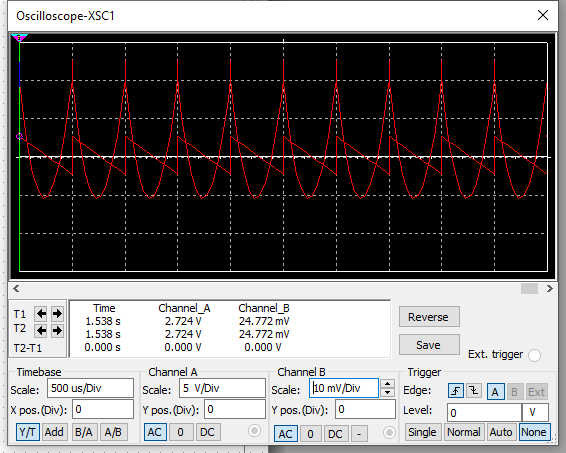
\includegraphics[width=0.75\linewidth]{/home/hxp/Notes/Physics_Experiment/近代物理实验——电路设计/微分电路/微分电路三角波有电阻有电容.png}
  \caption{微分电路三角波有电阻有电容}
\end{figure}

\begin{figure}[H]
  \centering
  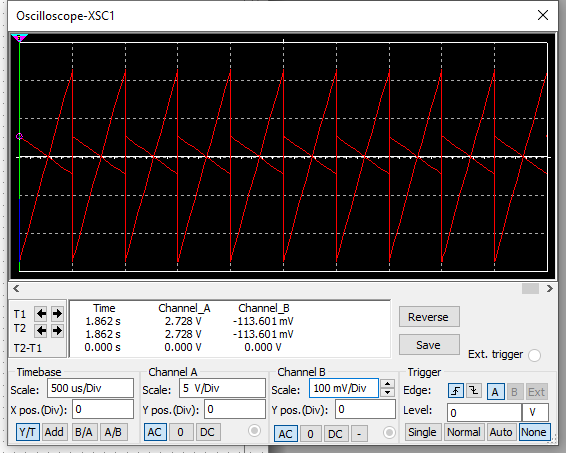
\includegraphics[width=0.75\linewidth]{/home/hxp/Notes/Physics_Experiment/近代物理实验——电路设计/微分电路/微分电路三角波有电阻无电容.png}
  \caption{微分电路三角波有电阻无电容}
\end{figure}

\begin{figure}[H]
  \centering
  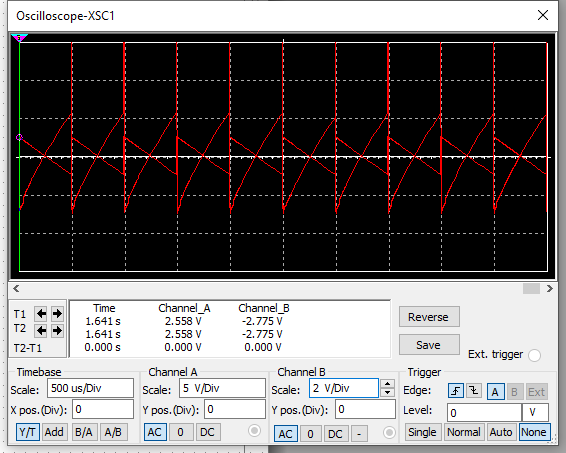
\includegraphics[width=0.75\linewidth]{/home/hxp/Notes/Physics_Experiment/近代物理实验——电路设计/微分电路/微分电路三角波无电阻有电容.png}
  \caption{微分电路三角波无电阻有电容}
\end{figure}

\begin{figure}[H]
  \centering
  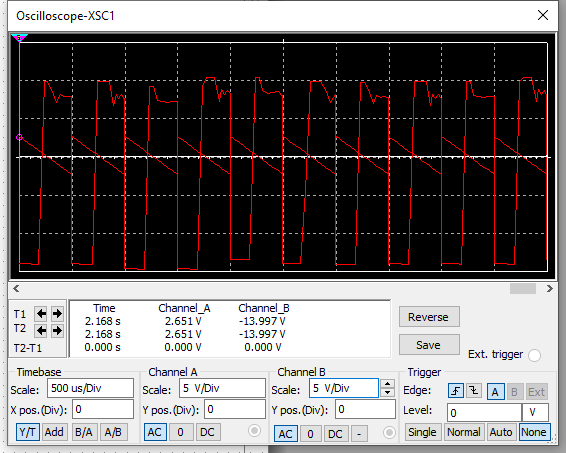
\includegraphics[width=0.75\linewidth]{/home/hxp/Notes/Physics_Experiment/近代物理实验——电路设计/微分电路/微分电路三角波无电阻无电容.png}
  \caption{微分电路三角波无电阻无电容}
\end{figure}

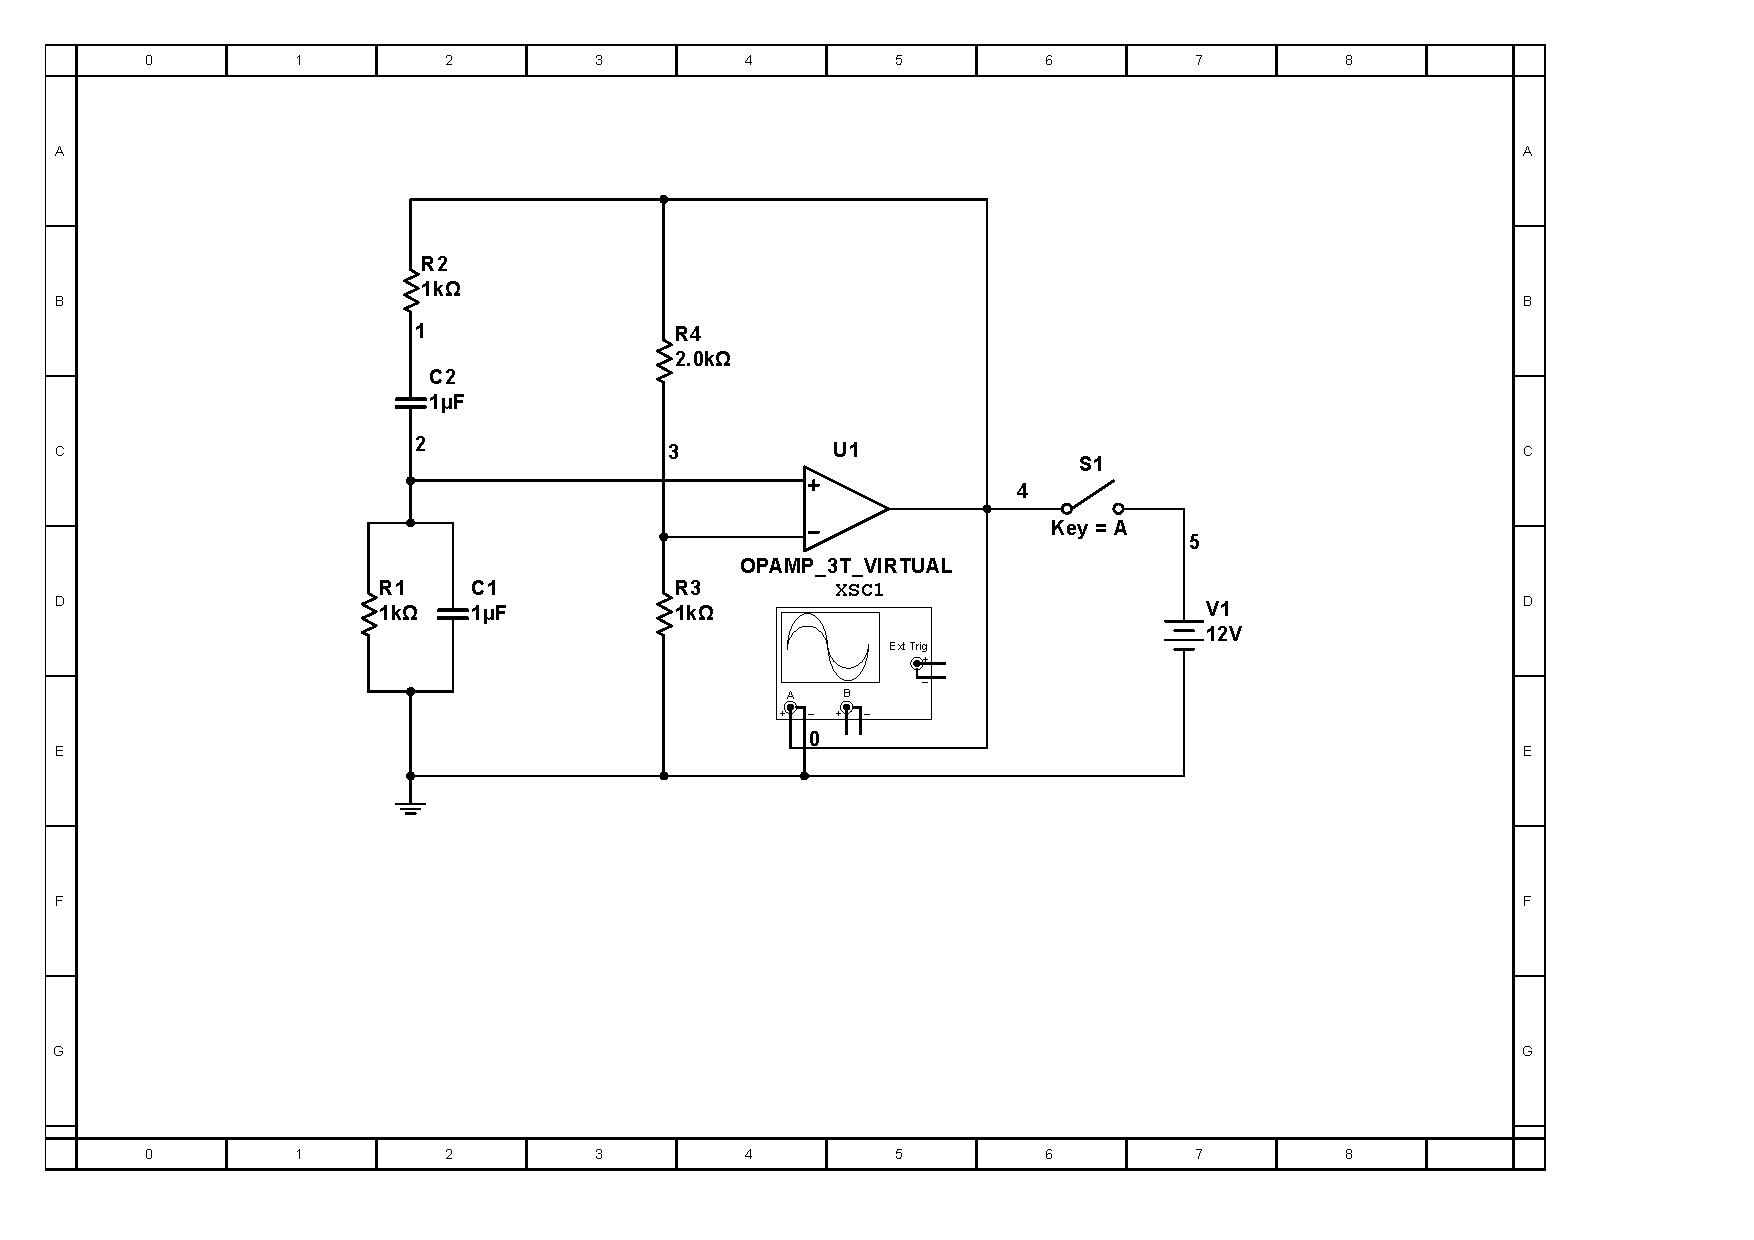
\includepdf[pages={1},angle=90]{/home/hxp/Notes/Physics_Experiment/近代物理实验——电路设计/正弦波发生器/正弦波发生器电路图.pdf}

\begin{figure}[H]
  \centering
  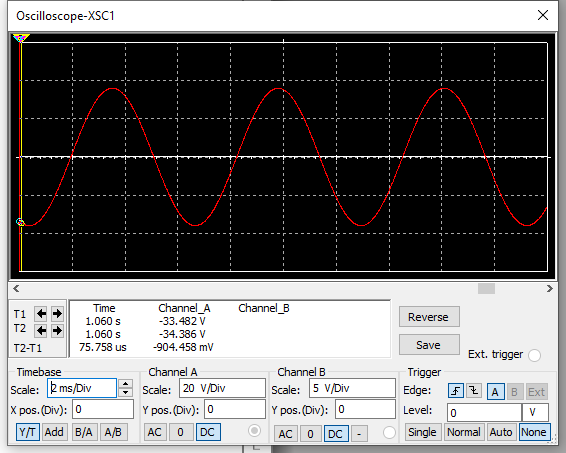
\includegraphics[width=0.75\linewidth]{/home/hxp/Notes/Physics_Experiment/近代物理实验——电路设计/正弦波发生器/正弦波发生器示波器.png}
  \caption{正弦波发生器}
\end{figure}

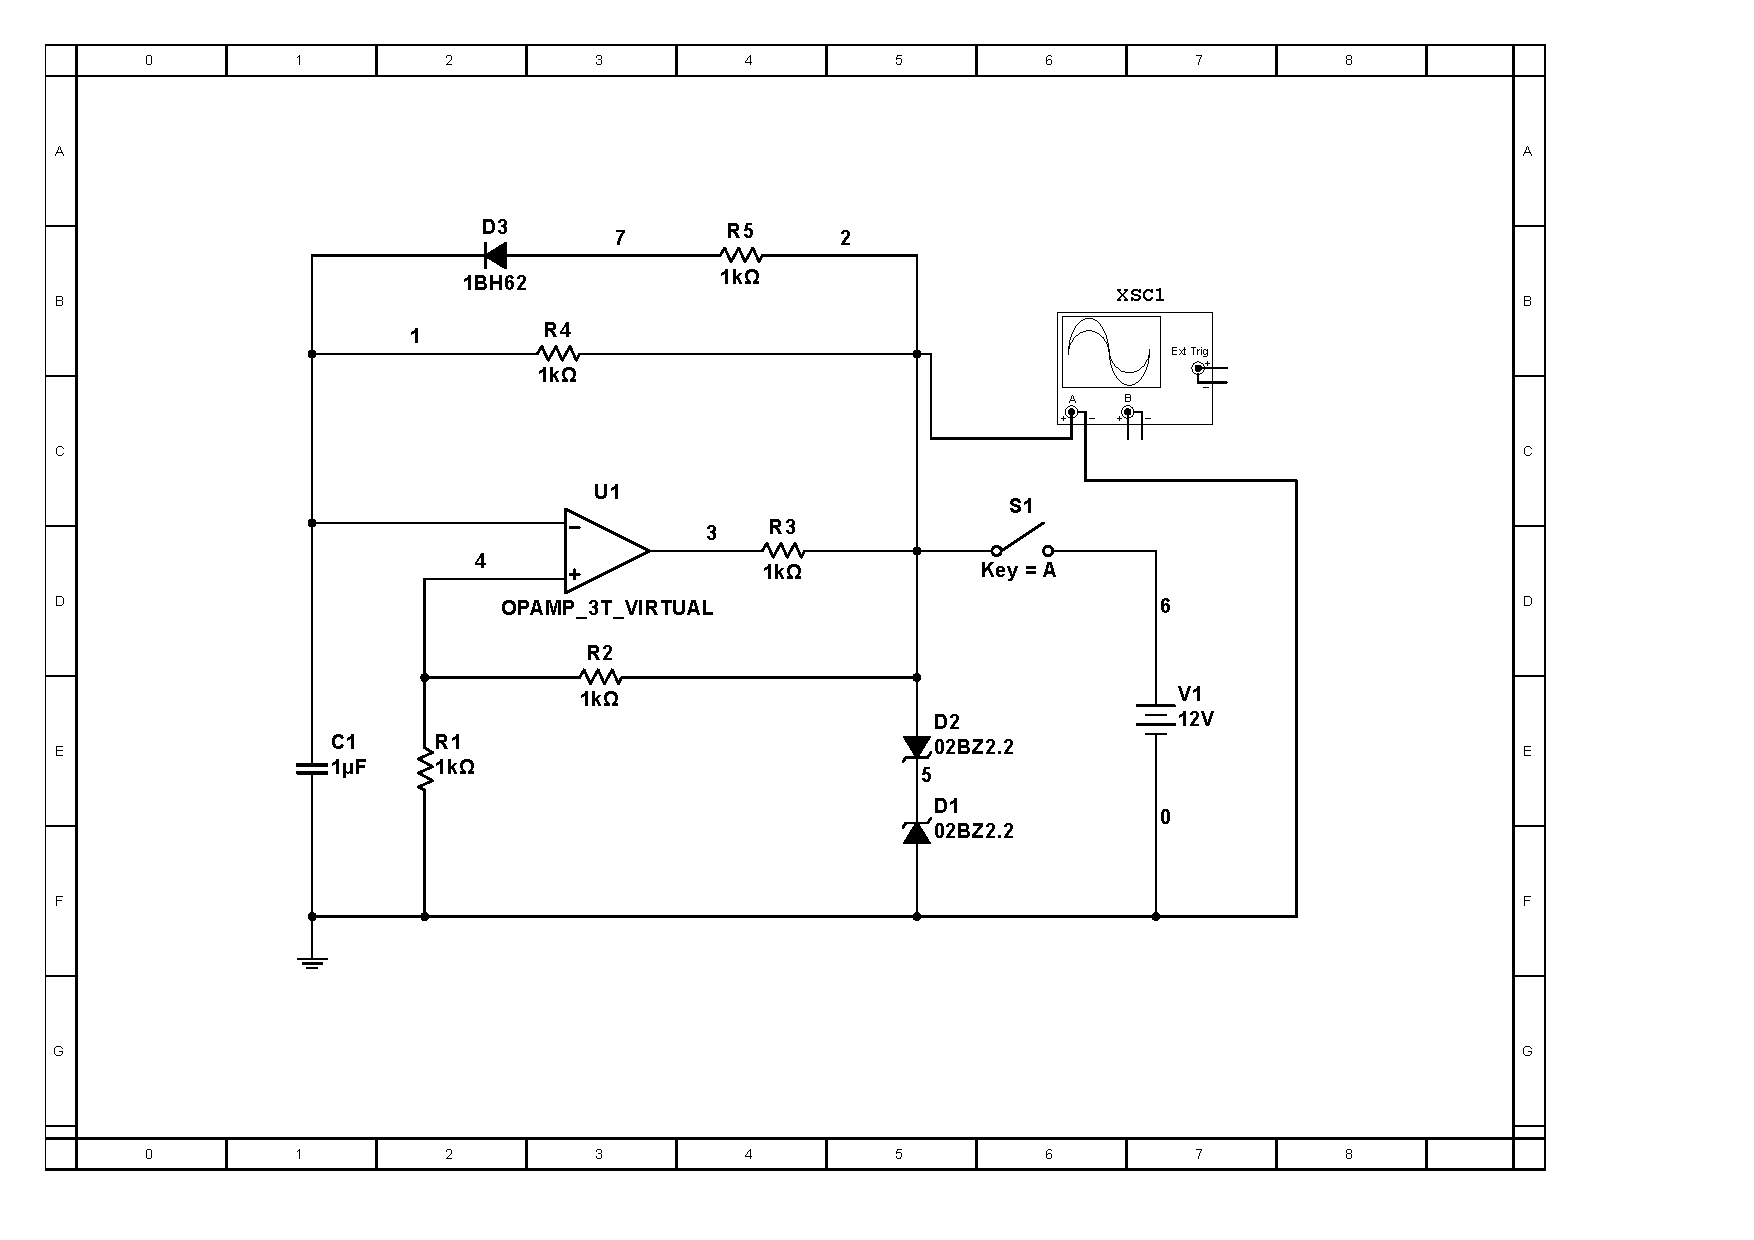
\includepdf[pages={1},angle=90]{/home/hxp/Notes/Physics_Experiment/近代物理实验——电路设计/矩形波电路/矩形波电路电路图.pdf}

\begin{figure}[H]
  \centering
  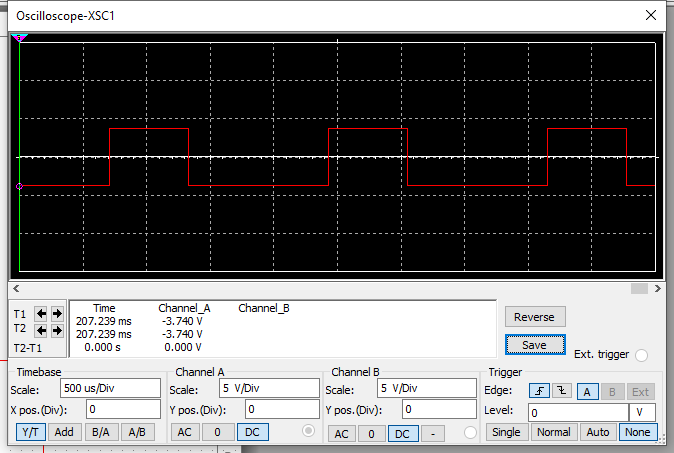
\includegraphics[width=0.75\linewidth]{/home/hxp/Notes/Physics_Experiment/近代物理实验——电路设计/矩形波电路/矩形波电路示波器图像.png}
  \caption{矩形波电路}
\end{figure}

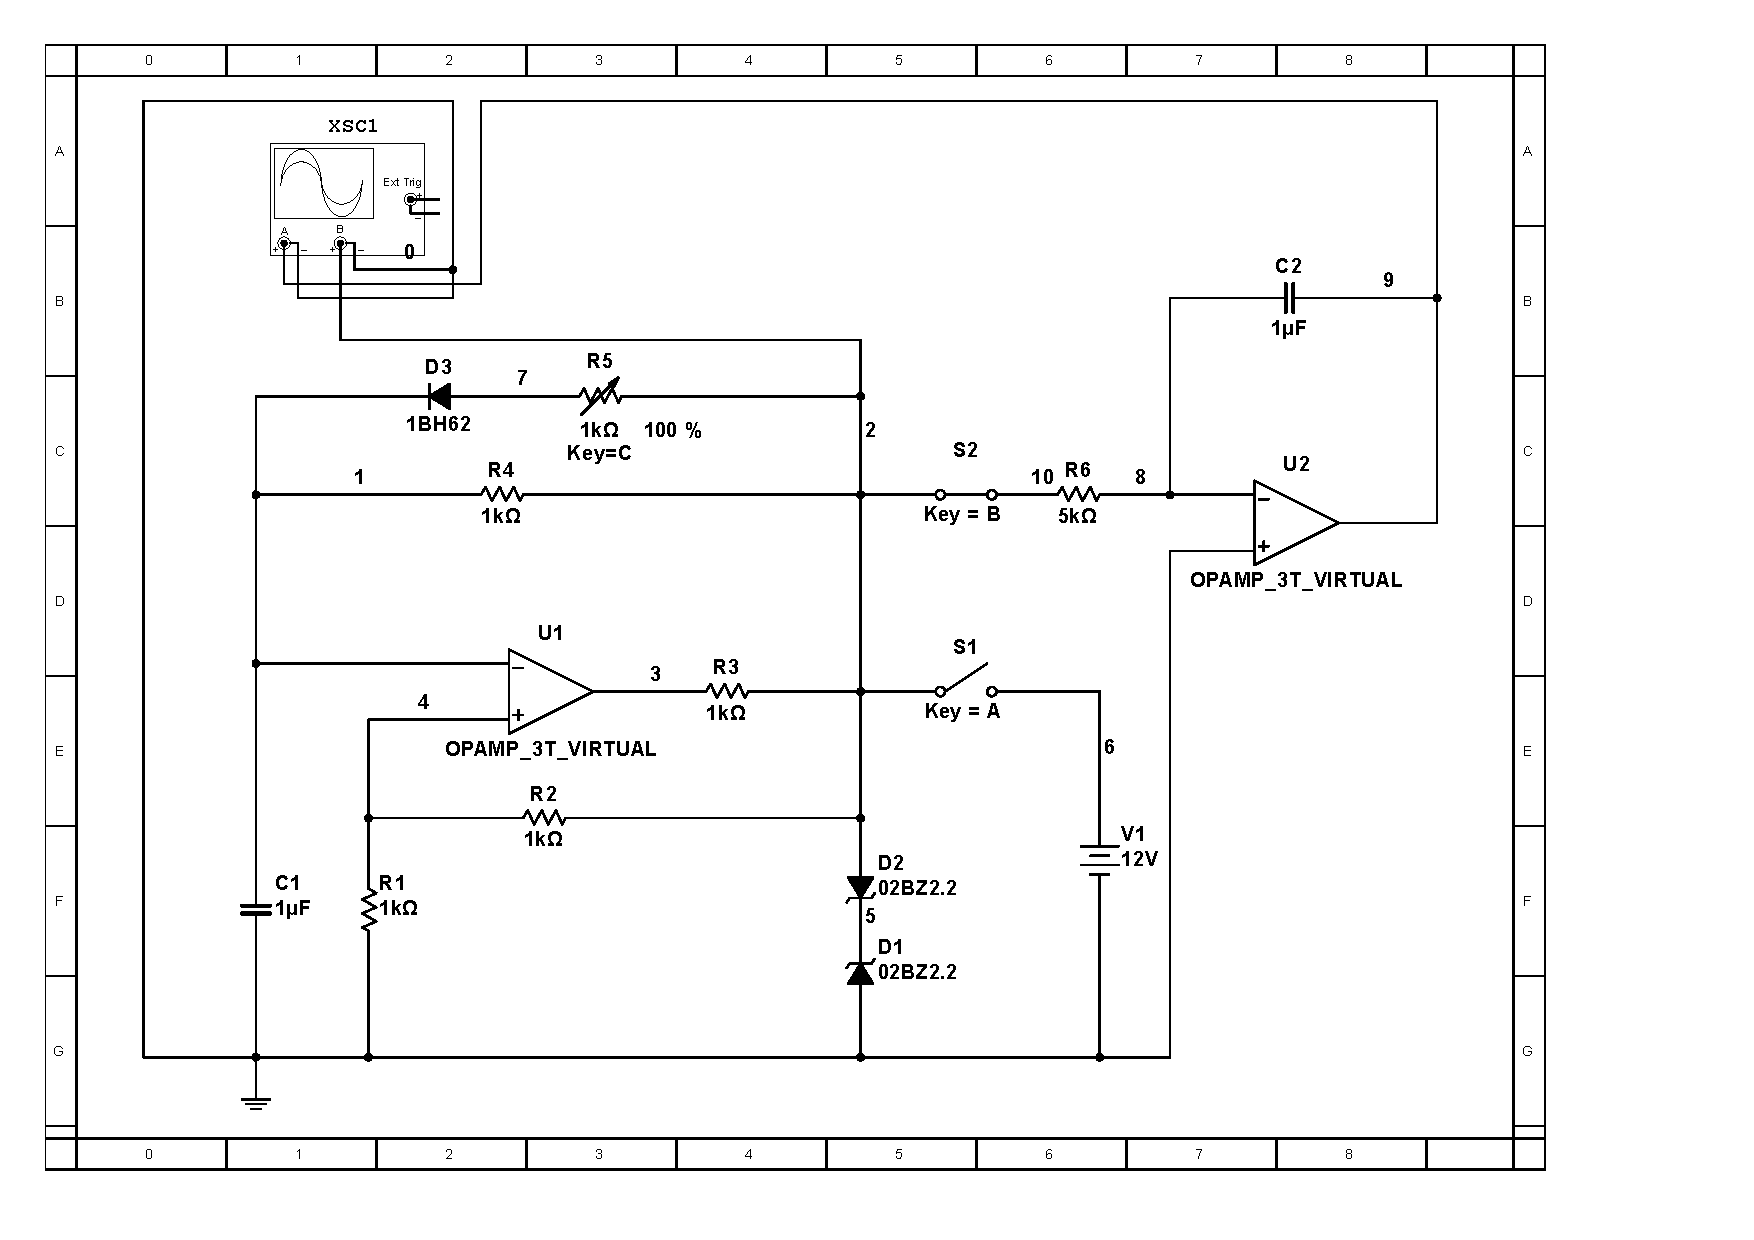
\includepdf[pages={1},angle=90]{/home/hxp/Notes/Physics_Experiment/近代物理实验——电路设计/矩形-三角波发生电路/矩形-三角波发生电路电路图.pdf}

\begin{figure}[H]
  \centering
  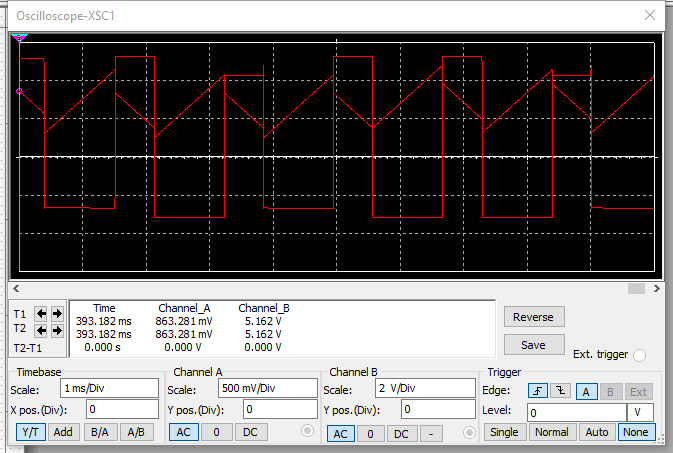
\includegraphics[width=0.75\linewidth]{/home/hxp/Notes/Physics_Experiment/近代物理实验——电路设计/矩形-三角波发生电路/矩形-三角波发生电路示波器.png}
  \caption{矩形-三角波发生电路}
\end{figure}

\end{document} 
